\documentclass[10pt]{beamer}

\usetheme[progressbar=frametitle]{metropolis}
\usepackage{appendixnumberbeamer}

\usepackage{booktabs}
\usepackage[scale=2]{ccicons}

\usepackage{pgfplots}
\usepgfplotslibrary{dateplot}

\usepackage{xspace}
\usepackage{minted}
%\usepackage{tabularx}
\usepackage{bytefield}
\newcommand{\themename}{\textbf{\textsc{metropolis}}\xspace}
\setminted[]{autogobble, breaklines, breakafter=-/,fontsize=\footnotesize}
\title{The C Language} 
\subtitle{CS238P: Operating Systems - Fall '18}
\author{Aftab Hussain\\ (Adapted from Vikram Narayanan's slides for ICS143A Fall'17)}
% \date{\today}
\date{October 12, 2018}
\institute{University of California, Irvine}
\begin{document}

\maketitle

\begin{frame}[standout]
  Data and Computation
\end{frame}

\begin{frame}{Data}
 Data can be of different types.
\begin{itemize}
\item char (1 byte)
\item int, long (4/8 bytes)
\item pointer (2, 4, or 8 bytes on x86 16, 32, and 64 bit machines respectively), structs, etc.
\end{itemize}
They can also be:
\begin{itemize}
\item constants
\item variables
\end{itemize}
\end{frame}

\begin{frame}{Data Variable}

  A data type therefore determines two things\footnote{https://www.tutorialspoint.com/cprogramming/c\_data\_types.htm}:

 \begin{itemize}
 \item the size of the data variable
 \item how the data is to be interpreted.
 \end{itemize}

 \end{frame}

 \begin{frame}[standout]
  Computation
\end{frame}

\begin{frame}{Statements}
\begin{itemize}
\item declarations
\item assignments
\item \texttt{for}, \texttt{do...while}, \texttt{while}
\end{itemize}
\end{frame}

\begin{frame}[fragile]{Hw1(xv6 shell)}
\begin{itemize}
\item<1-> \texttt{if...else}
\begin{minted}{c}
  pid = fork();
  if(pid == -1)
    perror("fork:");
\end{minted}
\item<2-> \texttt{switch...case}
\begin{minted}{c}
  switch(cmd->type){
  case '>': ...; break;
  default: ...; break;
  }
\end{minted}
\item<3-> Functions
\begin{itemize}
\item Process creation (\texttt{fork, exec})
\item File I/O (\texttt{open, close, read, write})
\end{itemize}
\end{itemize}
\end{frame}

\begin{frame}{Pointers}
  \begin{figure}
    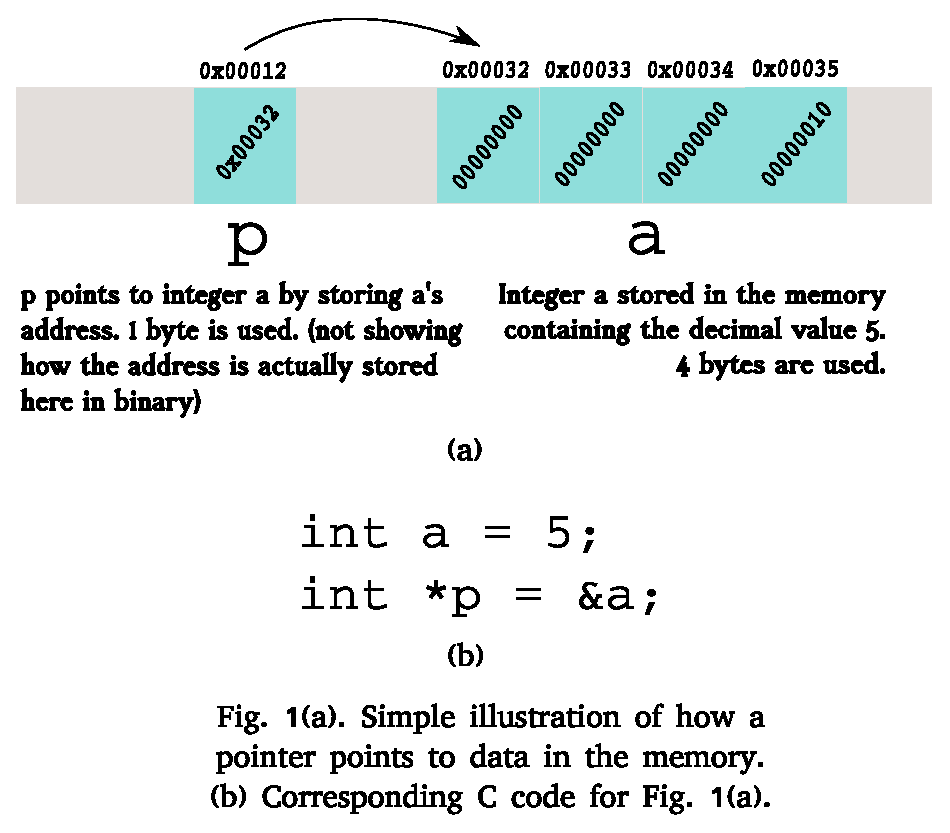
\includegraphics[scale=0.5]{figs/pointers.eps}
  \end{figure}
  \end{frame}

\begin{frame}[fragile]{Arrays}
\begin{itemize}
\item<1-> Collection of objects of the same data type
\item<2-> Accessed by index (\texttt{0 ... size - 1})
\item<3-> String is an array of characters 
\end{itemize}
\end{frame}

\begin{frame}[fragile]{Array Intialization}
Designated Initializers\footnote{http://gcc.gnu.org/onlinedocs/gcc-4.0.4/gcc/Designated-Inits.html}
\begin{minted}{c}
#define CAPSLOCK (1<<3)
#define NUMLOCK (1<<4)
#define SCROLLLOCK (1<<5)
static uchar togglecode[256] = {
[0x3A] CAPSLOCK,
[0x45] NUMLOCK,
[0x46] SCROLLLOCK
};
/* equivalent to */
togglecode[0x3A] = CAPSLOCK;
togglecode[0x45] = NUMLOCK;
togglecode[0x46] = SCROLLLOCK;
\end{minted}
Initialize the array elements 0x3A, 0x45, 0x46 only~\footnote{sheet 77, xv6-rev9.pdf}
\end{frame}

\begin{frame}[standout]
  Examples

  (arrays-ptrs.c \& arrays-strings.c)

\end{frame}


\end{document}
